% Copyright 2015  Ed Bueler

\documentclass[10pt,hyperref]{beamer}

\mode<presentation>
{
  \usetheme{Madrid}

  \usecolortheme{beaver}

  \setbeamercovered{transparent}
  
  \setbeamerfont{frametitle}{size=\large}
}

\setbeamercolor*{block title}{bg=red!10}
\setbeamercolor*{block body}{bg=red!5}

\usepackage[english]{babel}
\usepackage[latin1]{inputenc}
\usepackage{times}
\usepackage[T1]{fontenc}
% Or whatever. Note that the encoding and the font should match. If T1
% does not look nice, try deleting the line with the fontenc.

\usepackage{empheq}
\usepackage{animate}
\usepackage{xspace}
\usepackage{fancyvrb}
\usepackage{hyperref}



\title{Classical iterative methods for solving linear systems}

\author{Ed Bueler}

\institute{MATH 614 Numerical Linear Algebra}

\date{9 October 2015}



% If you wish to uncover everything in a step-wise fashion, uncomment
% the following command: 
%\beamerdefaultoverlayspecification{<+->}

\newcommand{\bb}{\mathbf{b}}
\newcommand{\bc}{\mathbf{c}}
\newcommand{\br}{\mathbf{r}}
\newcommand{\bx}{\mathbf{x}}
\newcommand{\by}{\mathbf{y}}
\newcommand{\bv}{\mathbf{v}}
\newcommand{\bu}{\mathbf{u}}
\newcommand{\bw}{\mathbf{w}}

\newcommand{\CC}{\mathbb{C}}
\newcommand{\RR}{\mathbb{R}}

\newcommand{\ddt}[1]{\ensuremath{\frac{\partial #1}{\partial t}}}
\newcommand{\ddx}[1]{\ensuremath{\frac{\partial #1}{\partial x}}}
\renewcommand{\t}[1]{\texttt{#1}}
\newcommand{\Matlab}{\textsc{Matlab}\xspace}
\newcommand{\Octave}{\textsc{Octave}\xspace}
%\newcommand{\MO}{\Matlab/\Octave}
\newcommand{\MO}{\Matlab}
\newcommand{\eps}{\epsilon}

\newcommand{\MS}{\alert{MAKE SURE}\xspace}

\newcommand{\exer}[2]{\medskip\noindent \textbf{#1.}\quad #2}

\newcommand{\mfile}[1]{
\VerbatimInput[frame=single,label=\fbox{\scriptsize \textsl{\,#1\,}},fontfamily=courier,fontsize=\scriptsize]{#1}
}

\newcommand{\mfiletiny}[1]{
\VerbatimInput[frame=single,label=\fbox{\scriptsize \textsl{\,#1\,}},fontfamily=courier,fontsize=\tiny]{#1}
}


\AtBeginSection[]
{
  \begin{frame}<beamer>
    \frametitle{Outline}
    \tableofcontents[currentsection,hideallsubsections]
  \end{frame}
}

\begin{document}

\begin{frame}
  \maketitle
\end{frame}


\begin{frame}{examples: two concrete linear systems}

\begin{itemize}
\item Suppose we want to solve the usual kind of linear system, namely
\begin{equation}
A \bx = \bb \label{introsystem}
\end{equation}
where $A\in \CC^{m\times m}$ and $\bb\in \CC^{m\times 1}$, to find $\bx\in \CC^{m\times 1}$.
\item  Throughout these notes we will use just two examples,
  \begin{itemize}
  \item[LS1] 
\begin{equation*}
\begin{bmatrix} 2 & 1 & 0 \\
                0 & 2 & 1 \\
                1 & 0 & 3 \end{bmatrix}
\begin{bmatrix} x_1 \\ x_2 \\ x_3 \end{bmatrix}
=
\begin{bmatrix} 2 \\ 1 \\ 4 \end{bmatrix}
\end{equation*}
  \item[LS2]
\begin{equation*}
\begin{bmatrix} 1 & 2 & 3 & 0 \\
                2 & 1 &-2 &-3 \\
               -1 & 1 & 1 & 0 \\
                0 & 1 & 1 &-1 \end{bmatrix}
\begin{bmatrix} x_1 \\ x_2 \\ x_3 \\ x_4 \end{bmatrix}
=
\begin{bmatrix} 7 \\ 1 \\ 1 \\ 3 \end{bmatrix}
\end{equation*}
  \end{itemize}
\item On the first problem in Assignment \#5 you will check that these are well-conditioned linear systems, and find their (unique) solutions.
\end{itemize}
\end{frame}


\begin{frame}{residual}

\begin{itemize}
\item By definition, the residual of a vector $\bx_0$ in linear system \eqref{introsystem} is the vector
\begin{equation}
\br_0 = \bb - A \bx_0. \label{residualdefn}
\end{equation}
  \vspace{-5mm}
  \begin{itemize}
  \item[$\circ$] Making the residual zero is the same as solving the system.
  \item[$\circ$] We call $\bx_0$ a ``test vector'' or ``approximate solution''.
  \end{itemize}

\bigskip
\item Evaluating the residual \eqref{residualdefn} requires a matrix-vector product and a vector subtraction.  This requires in total $O(m^2)$ operations at worst.
  \begin{itemize}
  \item[$\circ$] But many practical linear problems involve matrices $A$ for which the majority, often $99\%$ or more, of the entries are zero.\footnote{In such cases, $A^{-1}$ is generally \emph{dense}, i.e.~most entries are nonzero.}  Such a matrix is called \emph{sparse}.  The residual often requires $O(m)$ operations.
  \item[$\circ$] Thus, in many applications, evaluating the residual is much cheaper than applying Gauss elimination to solve linear system \eqref{introsystem}, which is an $O(m^3)$ operation in general.
  \end{itemize}
\end{itemize}
\end{frame}


\begin{frame}{Richardson iteration}

\begin{itemize}
\item \emph{Iterative methods} for linear system \eqref{introsystem} attempt to solve it by operations like computing the residual, or applying $A$ to a vector, plus other operations, to update the current vector approximation to $\bx$.
  \begin{itemize}
  \item[$\circ$] One wants the sequence of approximations, the iterates, to \emph{converge} to the solution $\bx = A^{-1} \bb$.
  \item[$\circ$] Iterative methods always require an initial iterate, the starting ``guess.''
  \end{itemize}
\item \emph{Richardson iteration}, sometimes called \emph{simple iteration}, adds a multiple $\omega$ of the last residual at each step,
\begin{equation}
\bx_{k+1} = \bx_k + \omega (\bb - A \bx_k).  \label{richardson}
\end{equation}
\item For system LS1, using initial iterate $\bx_0=0$ and $\omega=1/5$, \eqref{richardson} gives:\small
\begin{align*}
\bx_0 &= \begin{bmatrix} 0 \\ 0 \\ 0 \end{bmatrix}, \quad
\bx_1 = \begin{bmatrix} 0.4 \\ 0.2 \\ 0.8 \end{bmatrix}, \quad
\bx_2 = \begin{bmatrix} 0.6 \\ 0.16 \\ 1.04 \end{bmatrix}, \quad
\bx_3 = \begin{bmatrix} 0.728 \\ 0.088 \\ 1.096 \end{bmatrix}, \\
&\dots, \quad
\bx_{10} = \begin{bmatrix} 0.99817 \\ -0.01167 \\ 1.00667 \end{bmatrix}, \quad
\dots
\end{align*}
These iterates seem to be converging to $\bx = [1 \,\, 0 \,\, 1]^*$.
\end{itemize}
\end{frame}


\begin{frame}{eigenvalues and vectors}

Recall:
\begin{itemize}
\item A complex number $\lambda \in \CC$ is an \emph{eigenvalue} of a square matrix $B\in\CC^{m\times m}$ if there is a nonzero vector $\bv\in\CC^m$ so that $B \bv = \lambda \bv$.
\item The set of all eigenvalues of $B$ is the \emph{spectrum} $\sigma(B)$ of $B$.
\item The \emph{spectral radius} $\rho(B)$ is the maximum absolute value of an eigenvalue:
    $$\rho(B) = \max_{\lambda\in\sigma(B)}  |\lambda|$$
\item Even if $B$ is real, $\lambda$ may be complex.\footnote{The roots of a polynomial with real coefficients may be complex.}
\item Recall that \emph{singular values} are also eigenvalues:
    $$s \text{ is a singular value of } B \quad \iff \quad s \in \sigma(B^* B) = \sigma(B B^*)$$
\end{itemize}
\end{frame}


\begin{frame}{spectral properties and convergence of iterations}

\begin{itemize}
\item Properties of $B$ described in terms of its eigenvalues or singular values are generically called \emph{spectral properties}.  Some examples:
  \begin{itemize}
  \item[$\circ$] $\rho(B)$
  \item[$\circ$] $\sigma_1(B)=\|B\|_2$
  \item[$\circ$] the 2-norm condition number
    $$\kappa(B)=\|B\|_2/\|B^{-1}\|_2 = \sigma_1(B) / \sigma_m(B)$$
  \end{itemize}
\item \emph{the general idea}:  The conditions determining whether an iterative method for solving $A\bx = \bb$ converges, or not, generally depend on spectral properties of $A$ or associated matrices.
\item The right-hand side $\bb$ and the initial iterate $\bx_0$ generally do not determine whether the iteration converges, though a good choice of $\bx_0$ can speed up convergence.
\end{itemize}
\end{frame}


\begin{frame}{convergence of the Richardson iteration}

\begin{itemize}
\item Rewrite the Richardson iteration \eqref{richardson} as
\begin{equation}
    \bx_{k+1} = (I - \omega A) \bx_k + \omega \bb  \label{richardsonrewrite}
\end{equation}
\item The lemma on the next slide shows that Richardson iteration converges if and only if all the eigenvalues of the matrix on the right side of \eqref{richardsonrewrite} are inside the unit circle:
\begin{equation}
\text{\eqref{richardson} converges if and only if } \rho(I-\omega A) < 1.
\end{equation}

\item  Recall $\rho(B) \le \|B\|$ in any induced matrix norm---Exercise 3.2 in Trefethen \& Bau.  Thus \eqref{richardson} converges if $\|I-\omega A\| < 1$.
\end{itemize}
\end{frame}


\begin{frame}{convergence lemma}

\begin{lemma}  The iteration
   $$\by_{k+1} = M \by_k + \bc$$
converges to the solution of $\by = M \by + \bc$ for all initial $\by_0$ if and only if
   $$\rho(M) < 1.$$
\end{lemma}

\small
\begin{proof}
It is easy to solve this iteration by writing out a few cases:
\begin{align*}
   \by_2 &= M (M \by_0 + \bc) + \bc = M^2 \by_0 + (I + M) \bc, \\
   \by_3 &= M (M^2 \by_0 + (I + M) \bc) + \bc = M^3 \by_0 + (I + M + M^2) \bc,
\end{align*}
and so on.  By induction we get
    $$\by_k = M^k \by_0 + p_k(M) \bc$$
where $p_k(x) = 1 + x + x^2 + \dots + x^{k-1}$.  But $p_k(x) \to 1/(1-x)$ as $k\to\infty$ iff $x\in(-1,1)$.  Also, $\rho(M)<1$ iff $M^k \to 0$.  Thus $\by_k \to (I-M)^{-1} \bc$ iff $\rho(M) < 1$.
\end{proof}
\end{frame}


\begin{frame}[fragile]{the Richard iteration spectral condition}

\begin{itemize}
\item Since Richardson iteration converges if $\rho(I - \omega A)<1$ or $\|I-\omega A\|<1$, we choose $\omega$ based on the principle that
    $$\omega A \text{ should be close to the identity } I$$
\vspace{-5mm}
  \begin{itemize}
  \item[$\circ$] Not always possible!  Some matrices \emph{cannot} be rescaled to be close to $I$
  \end{itemize}

\medskip
\item We can graph $f(\omega) = \rho(I-\omega A)$:

\medskip
\begin{columns}
\begin{column}{0.5\textwidth}
\footnotesize
\begin{verbatim}
   omega = -1:.01:1;
   rho = zeros(size(omega));
   for j = 1:length(omega)
       M = eye(n) - omega(j) * A;
       rho(j) = max(abs(eig(M)));
   end
   plot(omega,rho)
\end{verbatim}

\smallskip
\begin{itemize}
\footnotesize
\item[LS1:]  $\rho(I - \omega A)$ dips below $1$ for $0 < \omega \lesssim 0.6$
\item[LS2:]  $\rho(I - \omega A) \ge 1$ always
\end{itemize}
\end{column}

\begin{column}{0.4\textwidth}
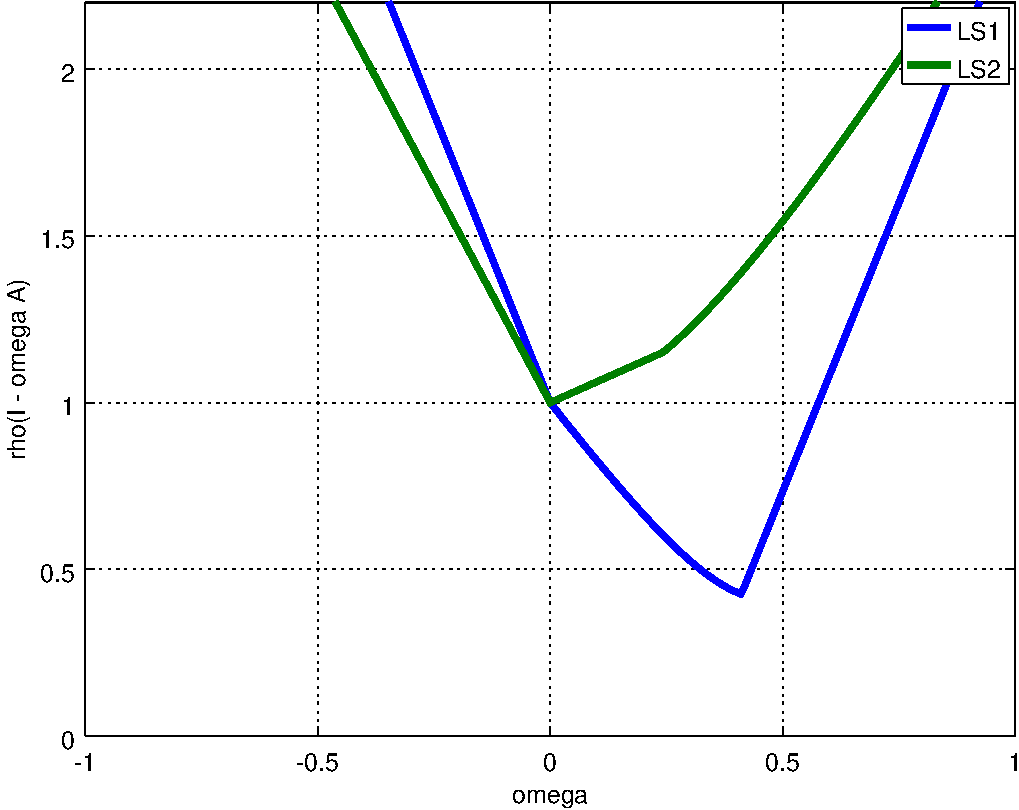
\includegraphics[width=2.0in,keepaspectratio=true]{richardspect}
\end{column}
\end{columns}

\medskip
\item  Note $\rho(I-0A)=1$ when $\omega=0$
\item  For LS1 we predict $\omega \approx 0.4$ gives fastest convergence.
\end{itemize}
\end{frame}


\begin{frame}{Jacobi iteration}

\begin{itemize}
\item Other classical iteration methods ``split'' the matrix $A$ before iterating.  The simplest is \emph{Jacobi iteration}.  It extracts the diagonal of $A$ and inverts it.
\item For this and the Gauss-Seidel iteration (next slide) we must assume

\centerline{\emph{all diagonal entries of $A$ are nonzero}: \quad  $a_{ii} \ne 0$}

\noindent This \emph{is} a restriction; many invertible matrices have zeros on the diagonal.

\item Split $A = D + L + U$ where $D$ is diagonal, $L$ is strictly lower triangular (so $\ell_{ij} = 0$ if $i \le j$), and $U$ is strictly upper triangular ($u_{ij} = 0$ if $i \ge j$).
\item The Jacobi iteration is
\begin{equation}
D \bx_{k+1} = b - (L + U) \bx_k  \label{jacobi}
\end{equation}
\item We could also write it \quad $\bx_{k+1} = D^{-1} \left(b - (L + U) \bx_k\right)$ \quad or as
\begin{equation*}
x_i^{(k+1)} = \frac{1}{a_{ii}} \left(b_i - \sum_{j\ne i} a_{ij} x_j^{(k)}\right)
\end{equation*}
where $x_j^{(k)}$ denotes the $j$th entry of the $k$th iterate $\bx_k$.
\end{itemize}
\end{frame}


\begin{frame}{Gauss-Seidel iteration}

\begin{itemize}
\item \emph{Gauss-Seidel iteration} extracts the non-strict lower-triangular part of $A$ and inverts it.
\item Again if $A = D + L + U$, with the same meanings as before, the Gauss-Seidel iteration is
\begin{equation}
(D + L) \bx_{k+1} = b - U \bx_k  \label{gaussseidel}
\end{equation}
\item We could also write it \quad $\bx_{k+1} = (D+L)^{-1} \left(b - U \bx_k\right)$ \quad \dots but that would miss the point!
\item Instead write it as \quad $D \bx_{k+1} = b - U \bx_k - L \bx_{k+1}$ \quad or equivalently:
\begin{equation}
x_i^{(k+1)} = \frac{1}{a_{ii}} \left(b_i - \sum_{j > i} a_{ij} x_j^{(k)} - \sum_{j < i} a_{ij} x_j^{(k+1)}\right)  \label{gaussseidelentrywise}
\end{equation}
\item Note the lower triangular entries apply to entries of $\bx_{k+1}$ which have already been computed.
\item Form \eqref{gaussseidelentrywise} is actually \emph{easier} to implement than Jacobi.
\end{itemize}
\end{frame}


\begin{frame}{convergence conditions for Jacobi and Gauss-Seidel}

\begin{itemize}
\item We know enough already to say that
  \begin{itemize}
  \item[$\circ$] Jacobi iteration converges if and only if $\rho(D^{-1} (L+U)) < 1$
  \item[$\circ$] Gauss-Seidel iteration converges if and only if $\rho((D+L)^{-1} U) < 1$
  \end{itemize}
\item However, these conditions are hard to use in practice, because computing these spectral radii (i.e.~maximum eigenvalues) is harder than solving the original system.
\item \emph{Definition}.  $A$ is \emph{strictly diagonally-dominant} if $|a_{ii}| > \sum_{j\ne i} |a_{ij}|$.
\item Two of the relatively-famous\footnote{Though I do not know who first proved these.}  theorems are these:
  \begin{itemize}
  \item[$\circ$] \emph{Theorem}.  Both the Jacobi and Gauss-Seidel iterations converge if $A$ is strictly diagonally-dominant.
  \item[$\circ$] \emph{Theorem}.  Gauss-Seidel iteration converges if $A$ is symmetric positive definite.
  \end{itemize}
\item Unlike the ``$\rho(\dots) < 1$'' conditions above, these are only \emph{sufficient} conditions.
  \begin{itemize}
  \item[$\circ$] E.g.~there are nonsymmetric $A$, which are \emph{not} diagonally-dominant, for which the iterations converge.
\end{itemize}
  \end{itemize}
\end{frame}


\begin{frame}{history, past and future}

\begin{itemize}
\item The Jacobi and Gauss-Seidel iterations are from the 19th century.
  \begin{itemize}
  \item[$\circ$] Probably Richardson was too, though it appears in a 1910 publication.
  \end{itemize}
\item The early history of numerical partial differential equations, e.g.~in the 1920 to 1970 period, heavily used these classical iterations.
  \begin{itemize}
  \item[$\circ$] A generalization of Gauss-Seidel iteration called \emph{successive over-relaxation}, was a particular favorite around 1970.
  \end{itemize}
\item But none of these iterations work on system LS2.
\item There are other iterative ideas, and they flourished in the 1990s.  One of the best known, ``GMRES'' from a 1992 paper, is in Lecture FIXME of Trefethen \& Bau.  It is in widespread use.  It works on LS2.
\item Iteration is the future:
  \begin{itemize}
  \item[$\circ$] It's obligatory on sufficiently-big systems.
  \item[$\circ$] It works better in parallel than direct methods.
  \end{itemize}
\end{itemize}
\end{frame}


\begin{frame}{biographies}

\begin{itemize}
\small
\item Gauss (1777--1855) did big stuff, while the Gauss-Seidel method is a small thing:

    \centerline{\href{https://en.wikipedia.org/wiki/Carl_Friedrich_Gauss}{\texttt{en.wikipedia.org/wiki/Carl\_Friedrich\_Gauss}}}

\medskip
\item Jacobi (1804--1851) was a major mathematician.  He also has his name on the ``Jacobian'', the matrix of derivatives appearing in Newton's method for systems of equations:

    \centerline{\href{https://en.wikipedia.org/wiki/Carl_Gustav_Jacob_Jacobi}{\texttt{en.wikipedia.org/wiki/Carl\_Gustav\_Jacob\_Jacobi}}}

\medskip
\item Richardson (1881--1953) is the most interesting.\footnote{To me, he is the best answer to ``Who was the last person to \emph{not} specialize and still be important in math and physics?''  Same for Gauss, and perhaps Jacobi, but they were earlier.}  He invented numerical weather forecasting, doing it by-hand for fun during WWI.  Later, as a pacifist and quaker, he quit the subject entirely when he found his meteorological work was of most value to chemical weapons designers and the British Air Force:

    \centerline{\href{https://en.wikipedia.org/wiki/Lewis_Fry_Richardson}{\texttt{en.wikipedia.org/wiki/Lewis\_Fry\_Richardson}}}

\medskip
\item Seidel (1821--1896) is relatively little known:

    \centerline{\href{https://en.wikipedia.org/wiki/Philipp_Ludwig_von_Seidel}{\texttt{en.wikipedia.org/wiki/Philipp\_Ludwig\_von\_Seidel}}}
\end{itemize}
\end{frame}

\end{document}

